\subsection{Quarto sprint}

\begin{minipage}{\textwidth}
  Di seguito è riportata la distribuzione delle ore per ciascun membro del team, accumulate in totali per persona e per ruolo:
  \begin{table}[H]
    \begin{tabularx}{\textwidth}{|c|*{6}{>{\centering}X|}c|}
      \hline
      \multicolumn{8}{|c|}{\textbf{Consuntivo orario}} \\
      \hline
      \textbf{Membro del team} & \textbf{Re} & \textbf{Am} & \textbf{An} & \textbf{Pt} & \textbf{Pr} & \textbf{Ve} & \textbf{Totale per persona} \\
      \hline
      Cavalli Riccardo & 0 & 0 & 0 & 0 & 3 & 5 & 8 \\ 
      \hline
      Pianon Raul & 0 & 0 & 7 & 0 & 0 & 1 & 8 \\ 
      \hline
      Dall’Amico Martina & 0 & 0 & 0 & 6 & 1 & 0 & 7 \\ 
      \hline
      Cristo Marco & 6 & 0 & 0 & 0 & 0 & 2 & 8 \\ 
      \hline
      Lewental Sebastiano & 0 & 6 & 0 & 0 & 0 & 1 & 7 \\ 
      \hline
      Zecchinato Mattia & 0 & 0 & 0 & 3 & 3 & 0 & 6 \\ 
      \hline
      Stocco Tommaso & 0 & 0 & 0 & 0 & 7 & 0 & 7 \\ 
      \hline
      \textbf{Totale ore per ruolo} & 6 & 6 & 7 & 9 & 14 & 9 & \textbf{51} \\
      \hline
    \end{tabularx}
    \caption{Sprint 4 - Consuntivo orario}
  \end{table}
  \end{minipage}
  
  \begin{figure}[H]
    \centering
    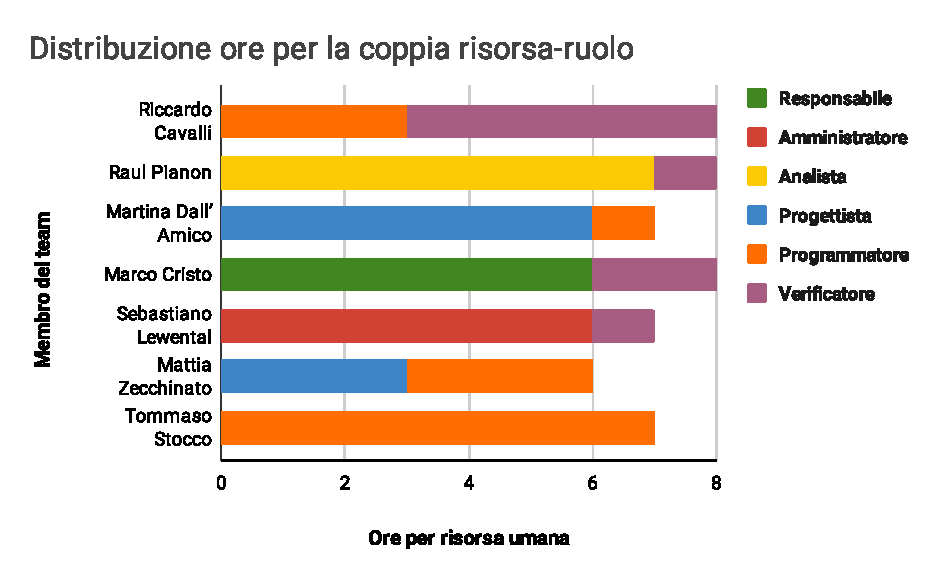
\includegraphics[width=0.90\textwidth]{assets/Consuntivo/Sprint-4/distribuzione_ore_risorsa_ruolo.pdf}
    \caption{Sprint 4 - Istogramma della distribuzione oraria per la coppia risorsa-ruolo}
  \end{figure}
  
  \begin{figure}[H]
    \centering
    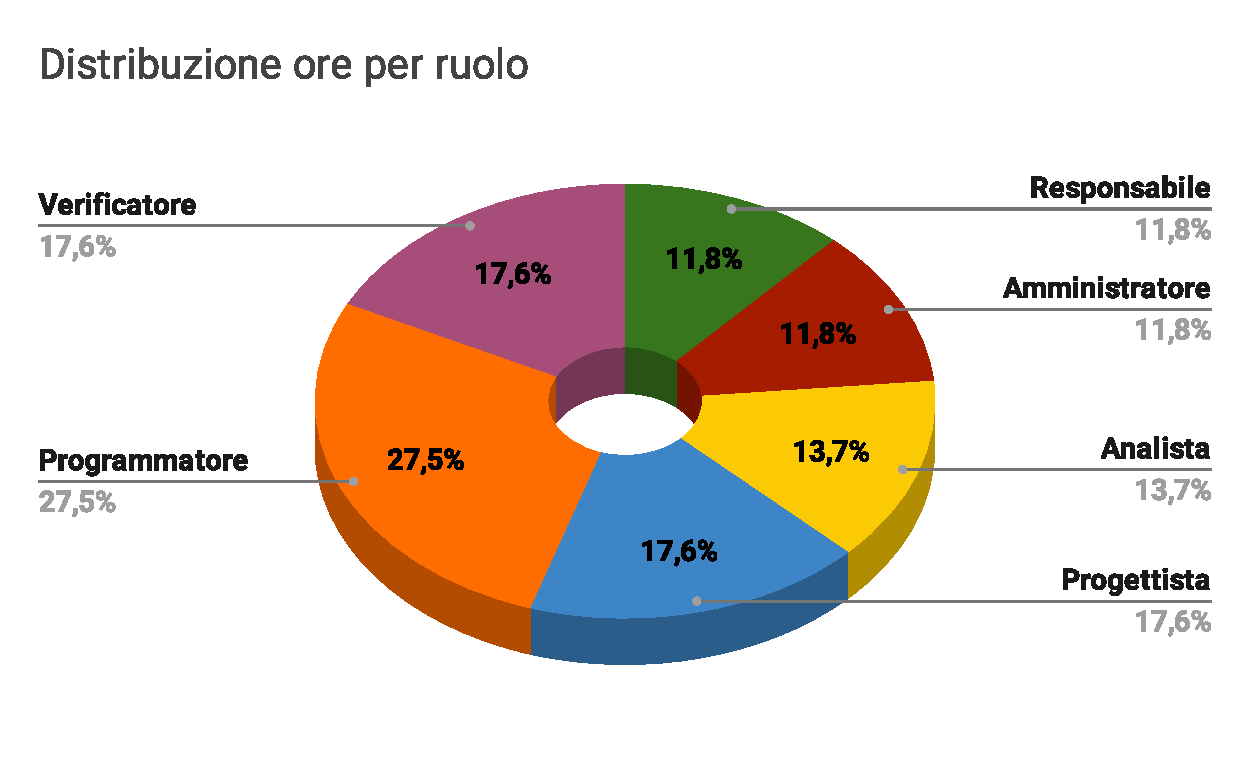
\includegraphics[width=0.90\textwidth]{assets/Consuntivo/Sprint-4/distribuzione_ore_ruolo.pdf}
    \caption{Sprint 4 - Areogramma della distribuzione oraria per ruolo}
  \end{figure}
  
  \begin{minipage}{\textwidth}
  Di seguito è riportato il consuntivo economico del quarto \glossario{sprint}:
  \begin{table}[H]
  \begin{adjustwidth}{-0.5cm}{-0.5cm}
    \centering
    \begin{tabular}{|P{2.9cm}|P{2.3cm}|P{2.5cm}|P{2.3cm}|>{\arraybackslash}P{2.5cm}|}
      \hline
      \multicolumn{5}{|c|}{\textbf{Consuntivo economico}} \\
      \hline
      \textbf{Ruolo} & \textbf{Ore per ruolo} & \textbf{Delta ore preventivo - consuntivo} & \textbf{Costo (in \texteuro)} & \textbf{Delta costo preventivo - consuntivo (in \texteuro)} \\
      \hline
      Responsabile & 6 & 0 & 180,00 & 0,00 \\ \hline
      Amministratore & 6 & 4 & 120,00 & 80,00 \\ \hline
      Analista & 7 & -1 & 175,00 & -25,00 \\ \hline
      Progettista & 9 & 0 & 225,00 & 0,00 \\ \hline
      Programmatore & 14 & -1 & 210,00 & -15,00 \\ \hline
      Verificatore & 9 & 1 & 135,00 & 15,00 \\ \hline
      \textbf{Totale} & \textbf{51} & 3 & \textbf{1.045,00} & 55,00 \\ \hline
      \textbf{Restante} & 444 & / & 8.710,00 & / \\ \hline
      \textbf{Sprint pregressi} & 149 & / & 3.230,00 & / \\ \hline
    \end{tabular}
    \caption{Sprint 4 - Consuntivo economico}
  \end{adjustwidth}
  \end{table}
  \end{minipage}
  
  \begin{figure}[H]
    \centering
    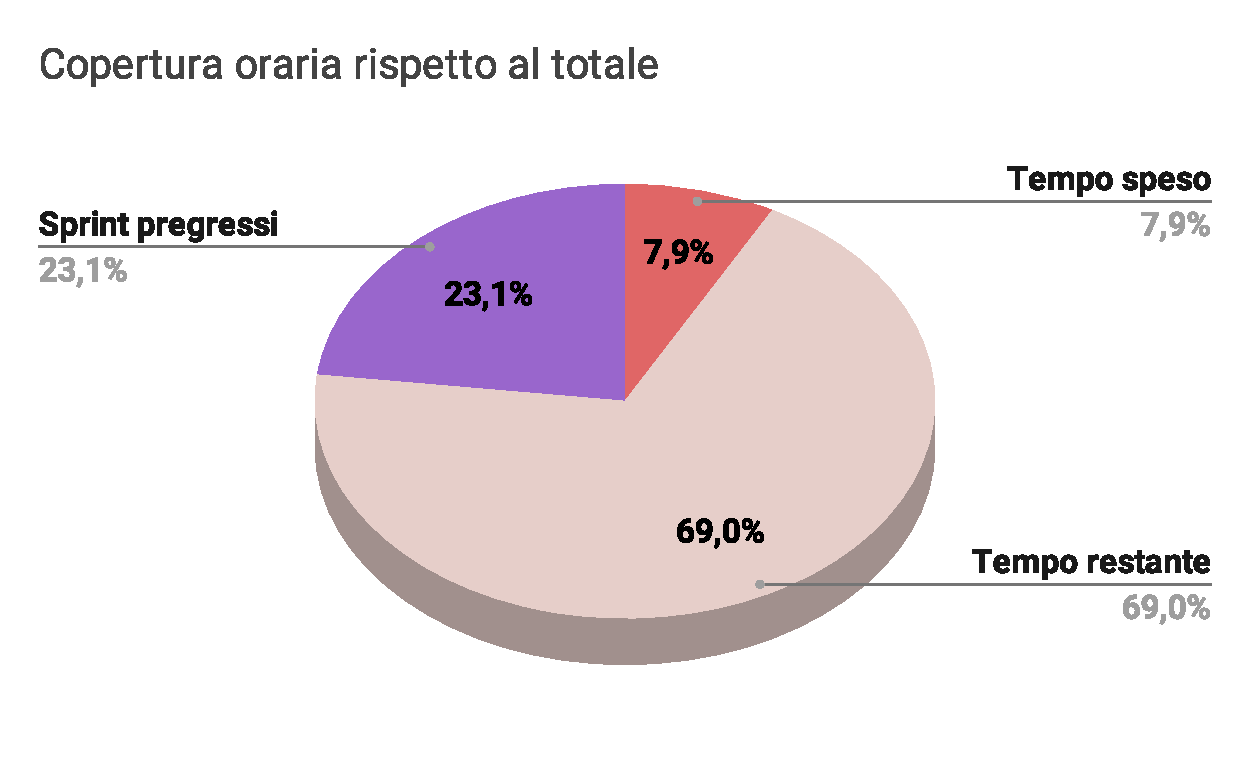
\includegraphics[width=0.90\textwidth]{assets/Consuntivo/Sprint-4/copertura_oraria.pdf}
    \caption{Sprint 4 - Areogramma del tempo speso (in ore) rispetto al totale}
  \end{figure}
  
  \begin{figure}[H]
    \centering
    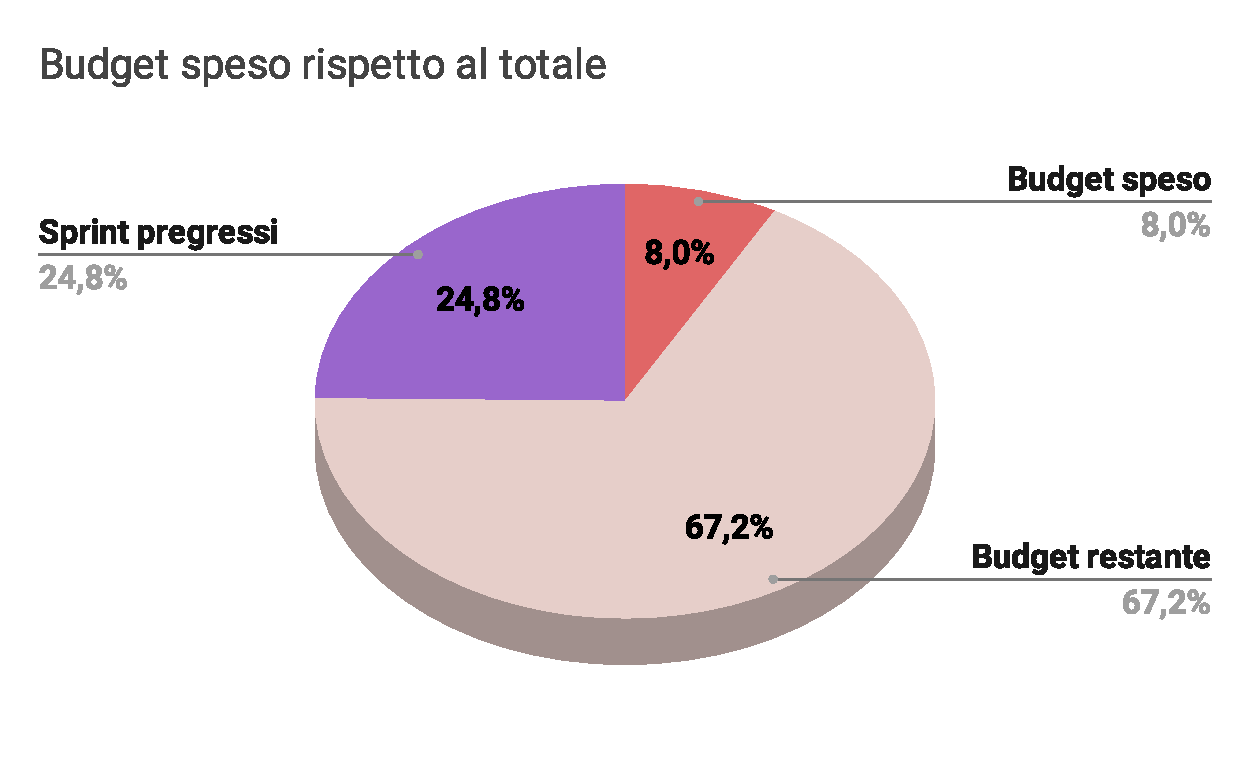
\includegraphics[width=0.90\textwidth]{assets/Consuntivo/Sprint-4/budget_speso.pdf}
    \caption{Sprint 4 - Areogramma del budget speso rispetto al totale}
  \end{figure}
  
  \begin{minipage}{\textwidth}
    Di seguito sono riportate le ore rimanenti per la coppia risorsa-ruolo:
    \begin{table}[H]
      \begin{tabularx}{\textwidth}{|c|*{6}{>{\centering}X|}c|}
        \hline
        \multicolumn{8}{|c|}{\textbf{Ore rimanenti per la coppia risorsa-ruolo}} \\
        \hline
        \textbf{Membro del team} & \textbf{Re} & \textbf{Am} & \textbf{An} & \textbf{Pt} & \textbf{Pr} & \textbf{Ve} & \textbf{Totale per persona} \\
        \hline
        Cavalli Riccardo & 0 & 2 & 9 & 14 & 18 & 16 & 59 \\ 
        \hline
        Pianon Raul & 2 & 10 & 2 & 20 & 15 & 12 & 61 \\ 
        \hline
        Dall’Amico Martina & 9 & 2 & 1 & 14 & 22 & 16 & 64 \\ 
        \hline
        Cristo Marco & 3 & 10 & 2 & 17 & 13 & 17 & 62 \\ 
        \hline
        Lewental Sebastiano & 9 & 4 & 2 & 11 & 21 & 17 & 64 \\ 
        \hline
        Zecchinato Mattia & 9 & 9 & 3 & 11 & 20 & 15 & 67 \\ 
        \hline
        Stocco Tommaso & 5 & 4 & 3 & 20 & 16 & 19 & 67 \\ 
        \hline
        \textbf{Totale ore per ruolo} & 37 & 41 & 22 & 107 & 125 & 112 & \textbf{444} \\ 
        \hline
      \end{tabularx}
      \caption{Sprint 4 - Ore rimanenti per la coppia risorsa-ruolo}
    \end{table}
  \end{minipage}

\subsubsection{Revisione delle attività}

Nell'arco del quarto \glossario{sprint}, il team ha svolto le seguenti attività:
\begin{itemize}
    \item Stesura verbali interni ed esterni;
    \item Revisione dei consuntivi pregressi all'interno del \PdP;
    \item Rielaborazione completa dei \glossario{casi d'uso} nell'\AdR;
    \item Estensione dei casi d'uso nell'\AdR\ in accordo con il team di programmatori;
    \item Creazione e connessione al database;
    \item Sviluppo dell'interfaccia di login tramite \glossario{Streamlit};
    \item \glossario{Dockerizzazione} dell'ambiente di sviluppo;
    \item Definizione dei test di correttezza del \glossario{prompt};
    \item Scelta definitiva del modello \glossario{LLM};
    \item Creazione della lista di selezione del dizionario dati;
    \item Sviluppo back-end della funzionalità di debug per il profilo Tecnico;
    \item Riorganizzazione del repository ChatSQL per integrare i moduli e rimuovere i file ridondanti;
    \item Refactoring completo del codice con rimozione dei file obsoleti;
\end{itemize}

\subsubsection{Retrospettiva}

\par Di seguito sono riportati i risultati del questionario di valutazione dello \glossario{sprint}:
\begin{itemize}
  \item Organizzazione dello \glossario{sprint}\ - Valutazione: 7;
  \item Conduzione dei meeting interni - Valutazione: 8;
  \item Conduzione dei meeting esterni - Valutazione: 8;
  \item Impegno e partecipazione dei singoli membri - Valutazione: 9;
  \item La quasi totalità dei membri del team era a conoscenza delle proprie mansioni;
  \item La numerosità delle riunioni è risultata adeguata per circa la metà dei membri, anche se il team preferirebbe organizzare più incontri informali tra programmatori;
  \item Le riunioni sono state organizzate quasi sempre con il giusto preavviso;
  \item Il rapporto ore spese/ore produttive è risultato meno ottimale dello \glossario{sprint} precedente;
  \item La produttività generale ha raggiunto una buona soglia;
  \item Alcuni membri del team ritengono opportuno avere più dettagli anche sulle task meno prossime.
\end{itemize}

\vspace{0.5\baselineskip}
\par A seguire le \textbf{analisi a posteriori} del quarto \glossario{sprint}:
\begin{itemize}
  \item La sola pianificazione iniziale delle attività non ha permesso ai membri del team di poter svolgere le proprie task a inizio \glossario{sprint}, richiedendo qualche giorno di stallo prima di potersi dedicare alle attività assegnate. Di conseguenza, il gruppo ha ritenuto opportuno, a partire dal prossimo sprint, che i ruoli uscenti spiegassero, tramite riunioni ad hoc, il lavoro che i ruoli entranti dovranno svolgere;
  \item Come conseguenza del punto precedente, il team ha stabilito di affidare l'assegnazione delle task per i ruoli entranti ai membri che non ricopreranno più lo stesso ruolo. In questo modo risulterà possibile delineare più puntualmente le attività imminenti;
  \item Anche se i risultati dei questionari di valutazione riguardo le riunioni mostrano una sufficiente adeguatezza organizzativa, il responsabile entrante ha ritenuto opportuno aumentare il margine di preavviso per minimizzare le assenze durante i meeting, comunicando il calendario delle riunioni future entro la fine dello sprint in corso;
  \item Nonostante si sia raggiunta una quantità apprezzabile di incontri informali tra membri dai ruoli affini durante la seconda metà dello sprint, lo stesso non si può dire per la prima settimana: questo ha portato ad alcuni periodi di ristagnamento nella prosecuzione delle attività, tenendo comunque alto l'impegno individuale e, di conseguenza, inficiando sul rapporto tra le ore spese e quelle produttive. Preso atto di ciò in vista della riunione di metà sprint, il team ha prontamente affrontato il problema e incrementato il numero di riunioni informative, recuperando così lo stallo iniziale.
\end{itemize}

\subsubsection{Aggiornamento pianificazione e preventivo}
\par Il team ha definito un piano d'azione per migliorare l'organizzazione e la produttività del prossimo \glossario{sprint}:
\begin{itemize}
  \item Aumentare il preavviso per i meeting futuri;
  \item I ruoli uscenti definiranno le task per i ruoli entranti nel corso dello \glossario{sprint};
  \item Incrementare il numero di riunioni informali;
  \item Effettuare una separazione più netta tra \glossario{front-end} e \glossario{back-end};
\end{itemize}

\paragraph*{Pianificazione futura:}

\paragraph*{Preventivo "a finire" (\sezione{sec:stima_temporale}):}
\par Data la numerosità delle risorse assegnate originariamente al ruolo di progettista, il team ha concordato la necessità della ridistribuzione di tali risorse a favore dell'amministratore, il cui impegno orario è stato ritenuto sottostimato, con un lieve aumento anche per i ruoli di programmatore e il verificatore. 
La ripartizione è avvenuta come segue:
\begin{itemize}
  \item Le ore complessive assegnate al ruolo di progettista sono diminuite da 161 a 140;
  \item Le ore complessive assegnate al ruolo di amministratore sono aumentate da 56 a 70;
  \item Le ore complessive assegnate al ruolo di programmatore sono aumentate da 154 a 161;
  \item Le ore complessive assegnate al ruolo di verificatore sono aumentate da 140 a 147;
\end{itemize}
Il monte ore individuali è di conseguenza aumentato da 91 a 92. Nonostante l'incremento delle ore totali per ruolo, la ridistribuzione delle risorse ha comportato un risparmio di €35.

\paragraph*{Gestione dei rischi (\sezione{sec:analisi_rischi}):}
\par Nel corso del quarto \glossario{sprint}, il team ha riscontrato l'affioramento dei seguenti rischi:
\begin{itemize}
  \item \textbf{Rischi relativi alla rotazione dei ruoli:} Diversi tra i membri del team hanno riscontrato disorientamento a seguito della rotazione dei ruoli. Una volta individuata tale problematica a seguito di confronti interni tra membri, è stata attuata la contromisura per quanto descritta nella \sezione{sec:analisi_rischi}. L'efficacia del metodo di mitigazione ha subito però una riduzione a causa della sua applicazione tardiva, causando un periodo di stagnamento iniziale.
\end{itemize}